
\section{Introduction}
\label{sec:introduction}


\paragraph{} The objective of this laboratory assignment is to build a BandPass Filter (BPF), this is, a circuit that allow frequencies with a certain range to pass but attenuate all others.
The specifications for this lab project are: a central frequency at 1000Hz and a gain at central frequency of 40dB.
 
Our circuit is comprised of a $\mu$A741 OPAMP connected to two resistors, creating a non-inverting amplifier, and a combination of resistors and capacitors to take care of the filtering, as it can 
be seen in figure 1.

\paragraph{} The signal gors through a first stage where a capacitor will block unwanted DC current and filter lower frequencies (this is the high pass filter). Next the signal goes through a combination of resistors and a $\mu$741 OPAMP. This arrangement creates 
a non-inverting amplifier. In this configuration, the output signal is "in-phase" with the input signal. Feedback control of the non-inverting OPAMP is achieved by applying a small part of 
the output voltage back to the inverting (-) terminal via R3-R4 voltage divider network. Finally, the signal goes through a voltage divider, made of resistor R2 and capacitor C2. The desired voltage corresponds to the voltage drop
 at the terminals of the capacitor which, as a result, is subjected to a low pass filtering. For this to run, we need two supply DC voltage sources 
overlapped with our main circuit in order to power the transistors inside the OPAMP.


\begin{figure}[h] \centering
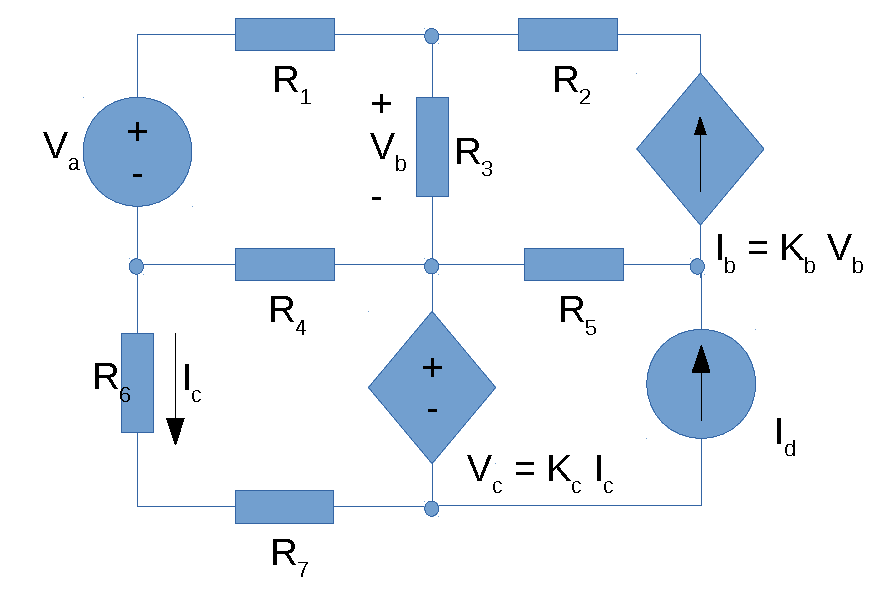
\includegraphics[width=0.7\linewidth]{circuit.pdf}
\caption{Geometry of our Band-Pass filter circuit.}
\end{figure}

\paragraph{} This report is subdivided into the following sections: Section 2, in which we layed out the theororical models and calculations used to determine the transfer fucntion and, consequentilly, the frequency response.
In Section 3 we display the results obtained in the simulation. Finally, in Section 4, we will compare both the theoretical results and draw conclusions.

\paragraph{} In the table below we display the values associated with each component used:

\begin{table}[h]
  \centering
  \begin{tabular}{|l|r|}
    \hline    
    {\bf Name} & {\bf Values} \\ \hline
    $R_1$ & 1.000000 kOhm \\ \hline 
$C_1$ & 0.220000 uFarad \\ \hline 
$R_2$ & 1.000000 kOhm \\ \hline 
$C_{21}$ & 0.220000 uFarad \\ \hline 
$C_{22}$ & 0.220000 uFarad \\ \hline 
$R_3$ & 1.000000 kOhm \\ \hline 
$R_{4a}$ & 100.000000 kOhm \\ \hline 
$R_{4b1}$ & 100.000000 kOhm \\ \hline 
$R_{4b2}$ & 100.000000 kOhm \\ \hline 
 
  \end{tabular}
  \caption{Values of components.}
  \label{tab:data}
\end{table}
